\graphicspath{ {img/23/} }

\chapter{Nevýhody súčasných metód}
\section{Podpora mobilných zariadení}

V roku 2010, Steve Jobs, spoluzakladateľ a~v tom čase aj výkonný riaditeľ Applu vydal vyhlásenie \emph{Thoughts on Flash}\cite{Apple_flash}, v~ktorom vysvetľuje prečo zariadenia iPhone, iPod a~iPad nepodporujú \emph{Adobe Flash}. Kritizuje \emph{Adobe Flash} z~uzavrenosti, vysokej systémovej záťaže, slabej bezpečnosti a~chýbajúcej podpore dotykových zariadení.
BBC v~roku 2012 informovala\cite{Android_flash}, že Adobe sťahuje \emph{Adobe Flash Player} z~\emph{Google Play store}, čo dovtedy umožňovalo prehrávať \emph{Adobe Flash} na~mobilných zariadeniach. To znamená, že mobilné operačné systémy, ktoré dohromady zaberajú 96,7\% trhu\cite{Mobile_OS_share} nepodporujú \emph{Adobe Flash}.


>> Zdroj hovorí len o~Smartphonoch, nie sú zahrnuté tablety. Použiť radšej: https://www.netmarketshare.com/operating-system-market-share.aspx?qprid=8&qpcustomd=1
>> Nenašiel som žiaden dobrý zdroj, ktorý by priamo vravel, že Silverlight nie je podporovaný na~iOS alebo Androide. Wikipedia rovno hovorí, že Silverlight je zastaraný. Opäť som ale nenašiel žiadne oficiálne tvrdenie.


\section{Zbytočné súbory na~serveri}

Nahrávanie obrázkov bez~toho, aby užívateľ najskôr obrázok videl, môže viesť k~tomu, že užívateľ nahraje nesprávny obrázok. Tak isto môže vzniknúť problém, kde užívateľ kvôli nesprávnemu spracovaniu obrázku na~serveri (napríklad nesprávny orez, pozri \ref{sec:orezanie-obrazka}), môže zmeniť svoje rozhodnutie. Takto vznikajú na~serveri súbory - obrázky, ktoré sa nikdy nepoužijú. Jedno z~riešení tohto problému je pravidelné mazanie nevyužívaných obrázkov.   

\section{Orezanie obrázka}
\label{sec:orezanie-obrazka}

Pri spracovaní na~serveri zvyčajne dochádza k~zmenšeniu a~orezaniu obrázka. Spravidla sa obrázky orezávajú na~stred. To však môže byť nesprávne, ako ukazuje obrázok XX (TODO), kde orezanie na~stred odreže osobu - najdôležitejšiu časť obrázka. Čiastočným riešením je využitie detekcie tvárí. Pokročilé riešenia si však vyžadujú pokročilú analýzu obrazu, kde sa analyzuje kontrast a~hrany. Vďaka tomu je možné detekovať východ slnka, alebo budovu na~obrázku. 

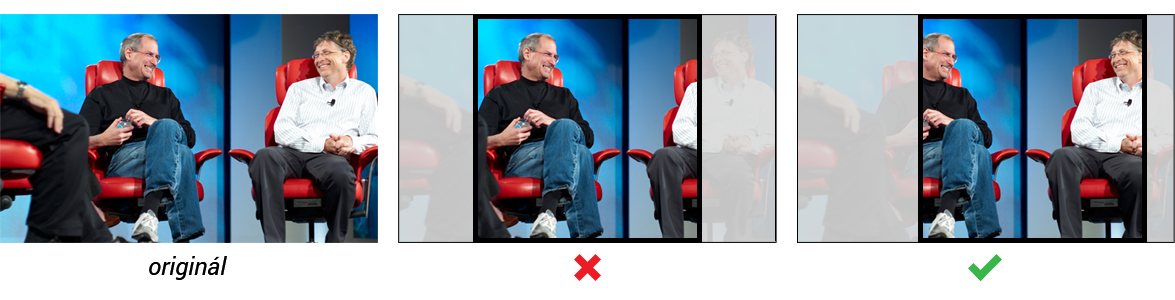
\includegraphics[width=\textwidth]{jobs_gates}

\section{Prenášanie zbytočných dát}

// TODO